\chapter{Results}

In this chapter we present the results of the data collection heuristic
proposed in chapter~3. The heuristic used for simulation, as stated 
earlier, ignores $t_{LS}$ and $t_{MBS}$. %what are these quantities?
%% The intro to chater must tell the reader what to expect in chapter.
%% But the summary here start abruptly. How simulation is planned?
%% No mention about the parameters of simulation or how realistic their
%% choices are.

We now present simulation results of our heuristic applied on the following cases:
\begin{itemize}
\item Field size 1000m $\times$ 1000m
\item Sensor Range: 50 m
\item Number of sensors: 50, 60, 70, 80, 90, 100
\end{itemize}

\subsection{50 sensors}
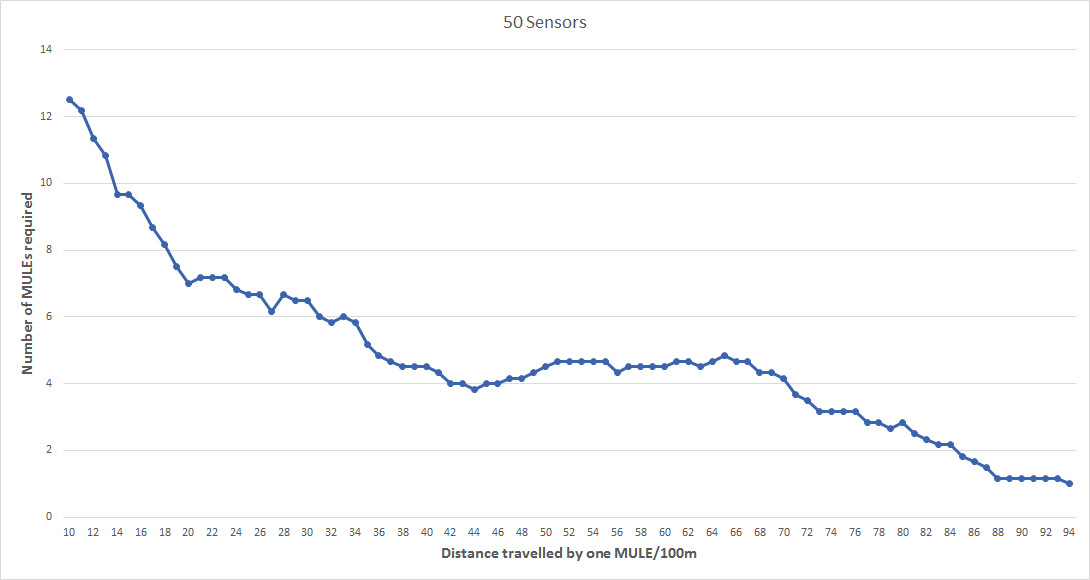
\includegraphics[width=15cm]{50_avg}
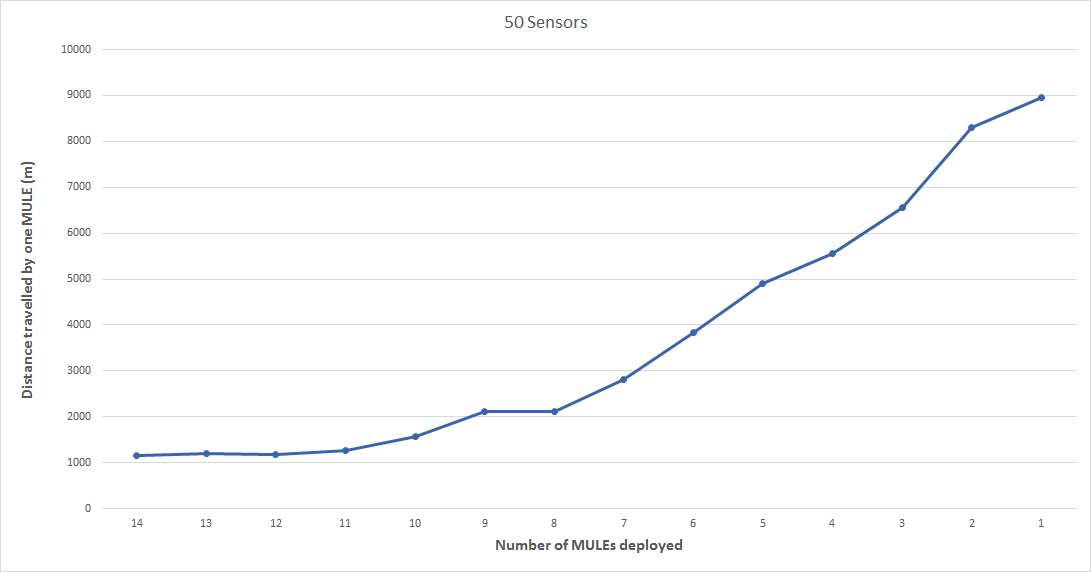
\includegraphics[width=15cm]{50_lat}

\subsection{60 sensors}
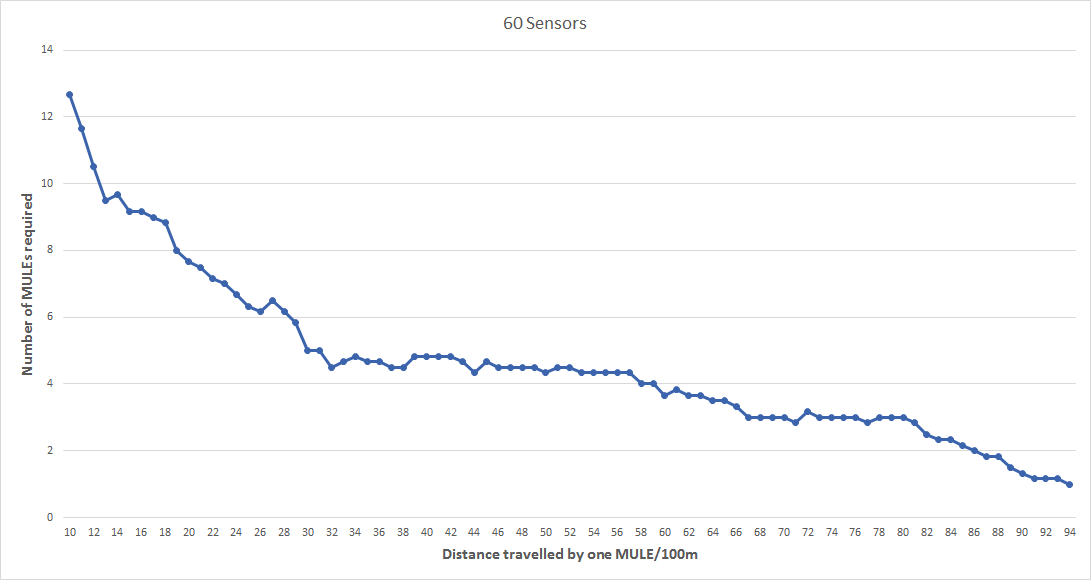
\includegraphics[width=15cm]{60_avg}
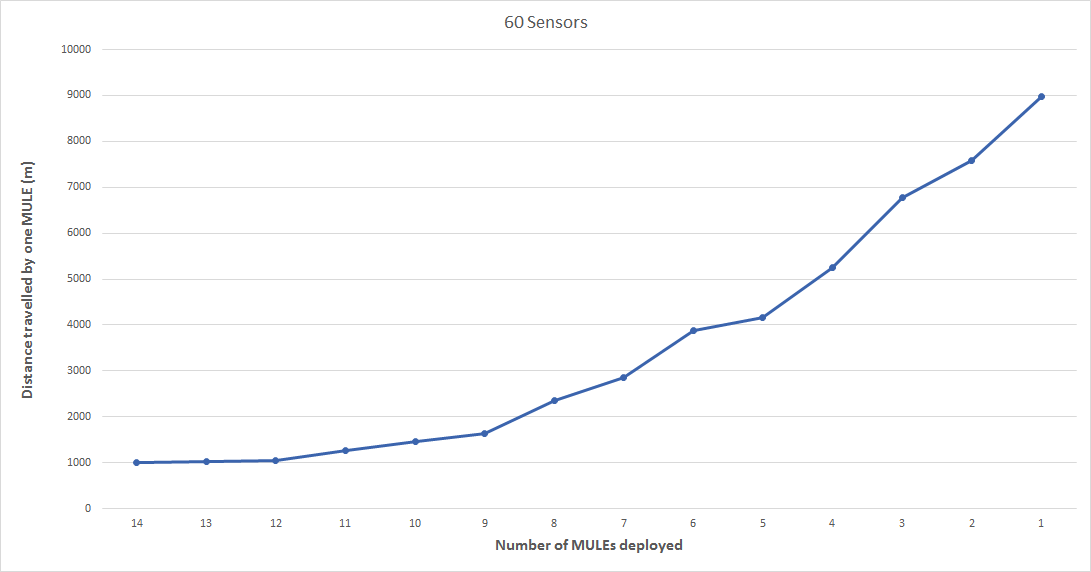
\includegraphics[width=15cm]{60_lat}

\subsection{70 sensors}
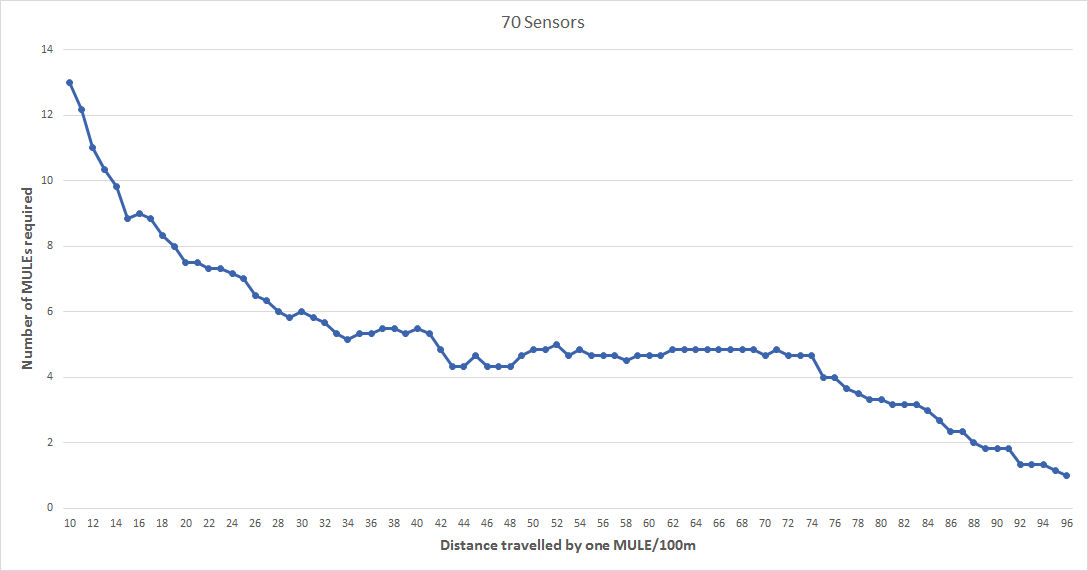
\includegraphics[width=15cm]{70_avg}
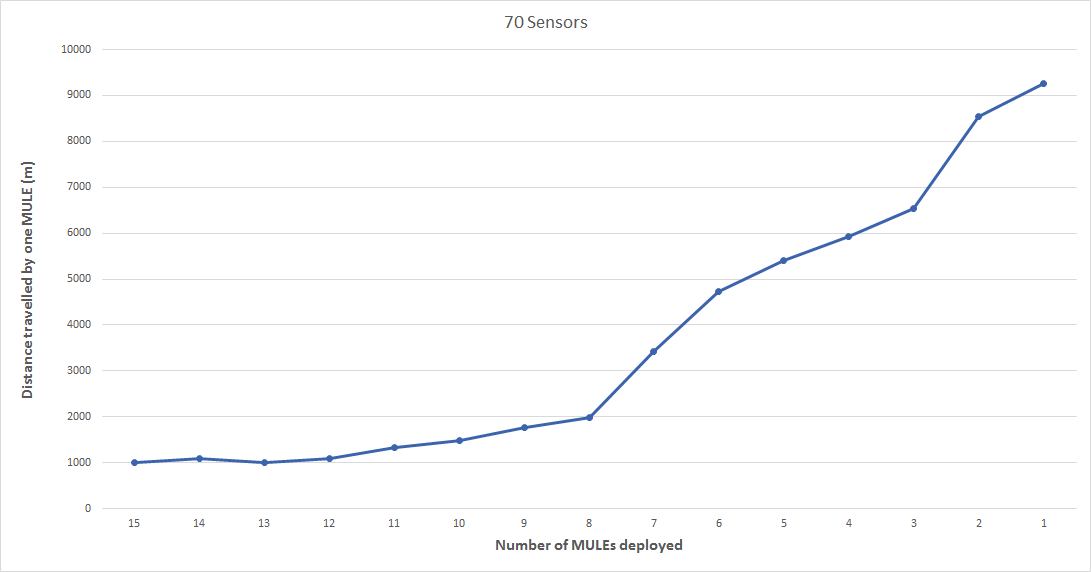
\includegraphics[width=15cm]{70_lat}

\subsection{80 sensors}
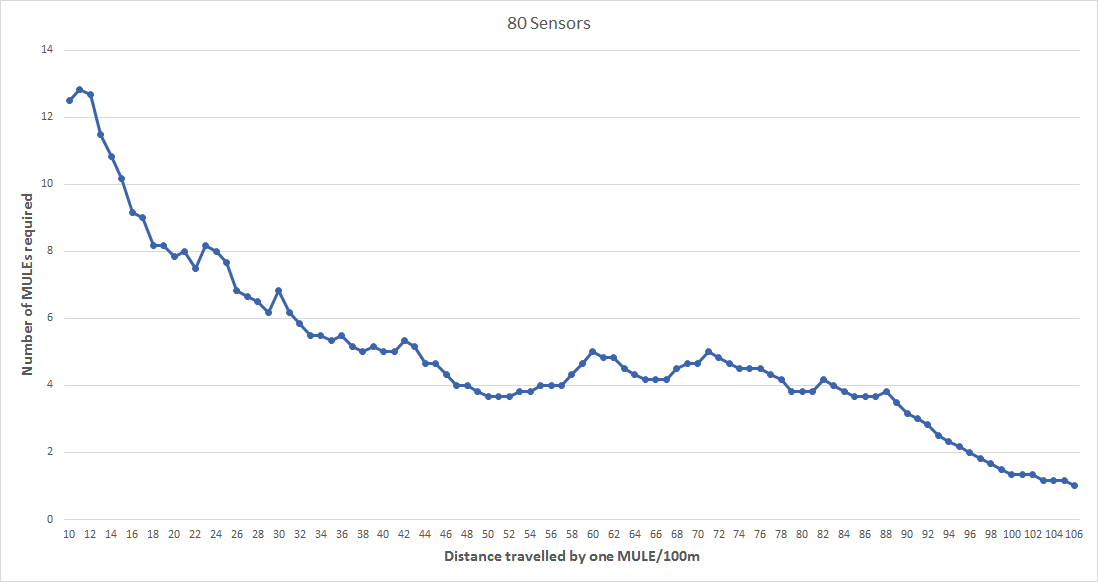
\includegraphics[width=15cm]{80_avg}
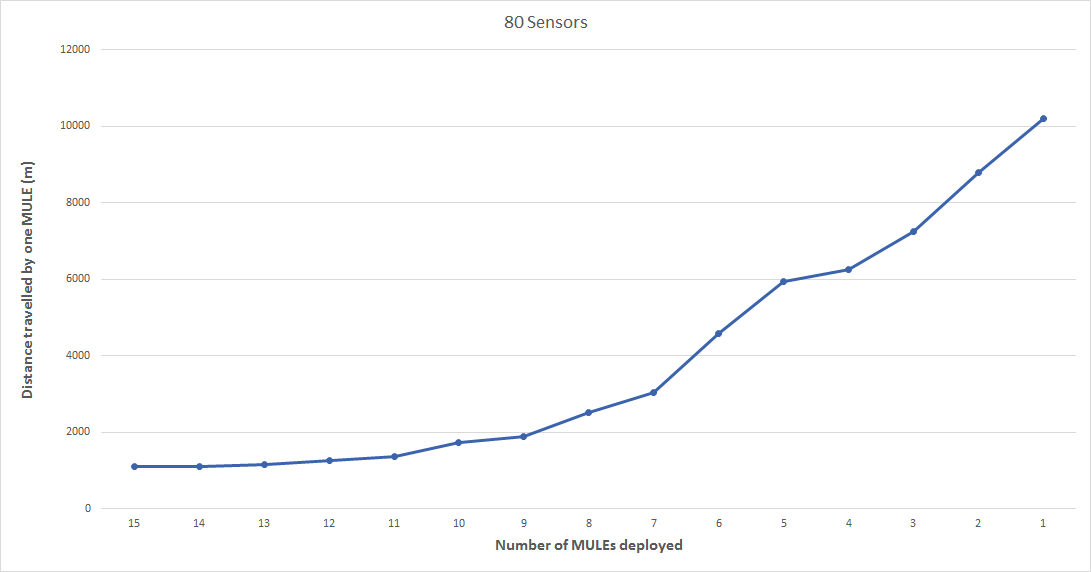
\includegraphics[width=15cm]{80_lat}

\subsection{90 sensors}
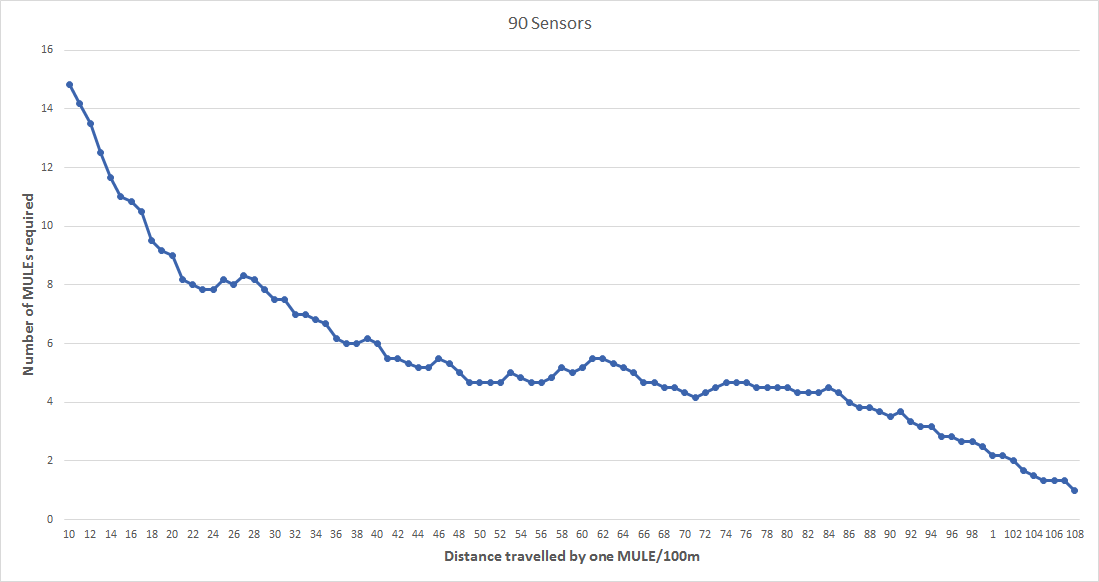
\includegraphics[width=15cm]{90_avg}
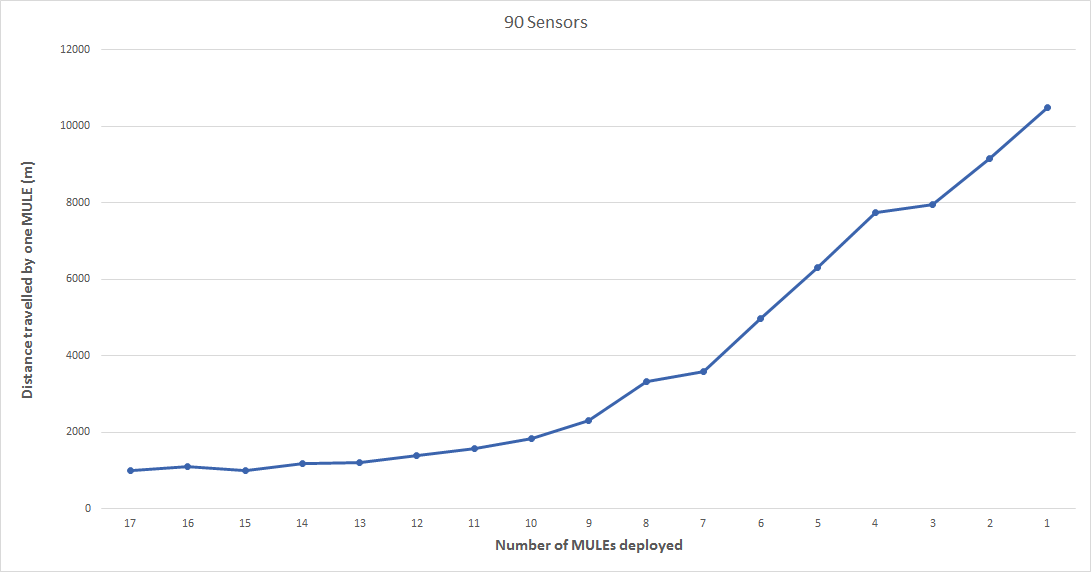
\includegraphics[width=15cm]{90_lat}

\subsection{100 sensors}
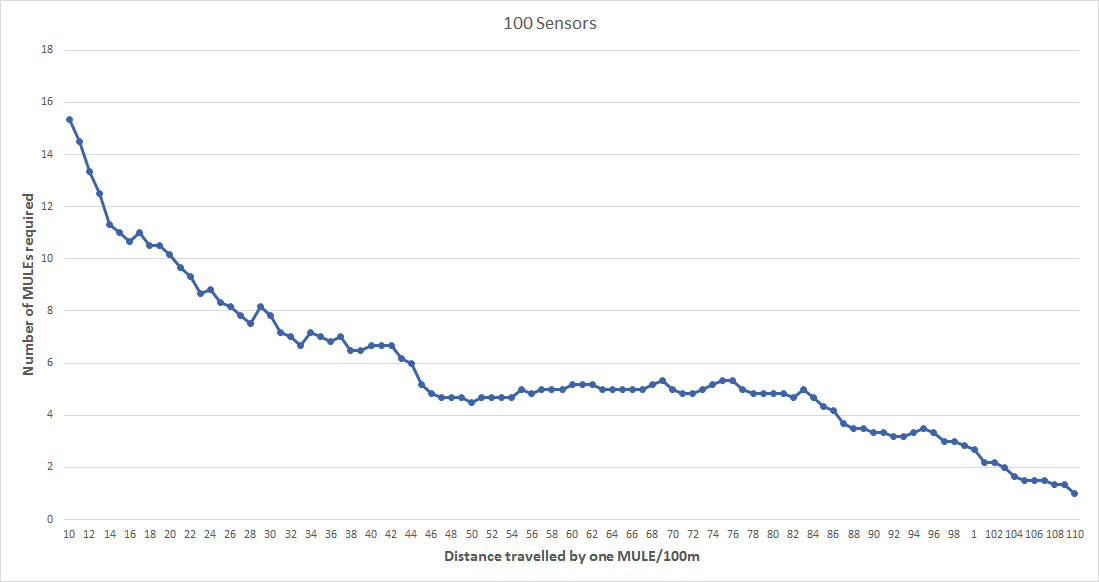
\includegraphics[width=15cm]{100_avg}
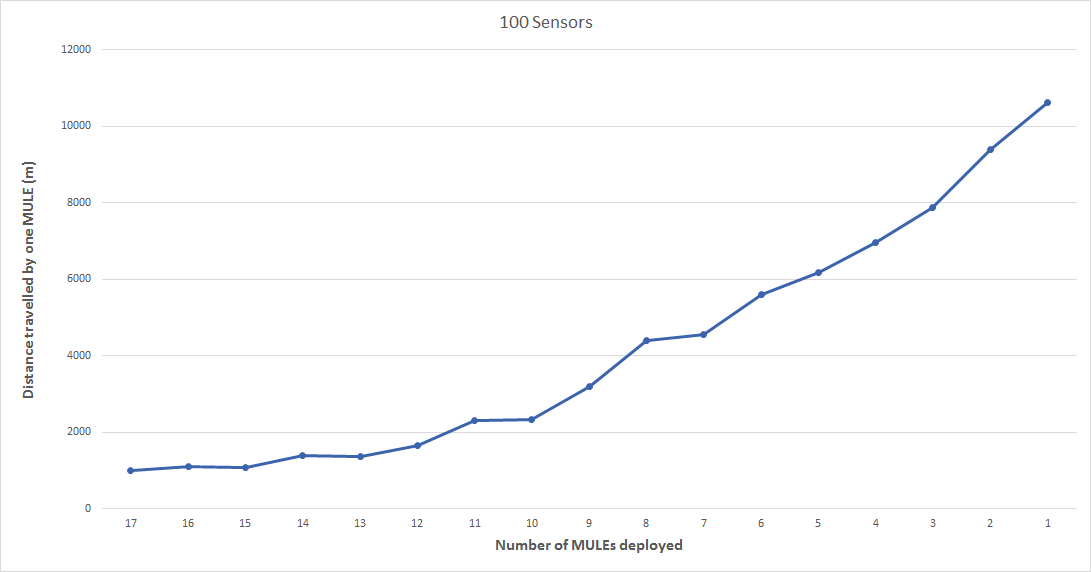
\includegraphics[width=15cm]{100_lat}
